% !TEX encoding = UTF-8
% !TEX TS-program = pdflatex
% !TEX root = ../tesi.tex

%**************************************************************
\chapter{Contesto Aziendale}
\label{cap:contesto-aziendale}
%**************************************************************

\section{L'azienda}
\subsection{Descrizione}
Le informazioni a seguito sono state prese direttamente dall'azienda, tuttavia ritengono siano rappresentative della realtà considerando sia il progetto al quale ho partecipato, sia il resto dell'offerta \textit{software}.\\
\textbf{Datasoil S.r.l.} è una \textit{startup} che si occupa di sviluppare applicativi dedicati alla gestione aziendale, altamente integrati con industria 4.0 e \textit{digital twin} (controparte digitale di un oggetto reale, ad esempio un macchinario di una linea produttiva): vengono impiegati apprendimento automatico\footnote{Anche detto \textit{machine learning} in inglese è una branca dell'intelligenza artificiale che utilizza metodi statistici per migliorare la performance di un algoritmo nell'identificare pattern nei dati, nella quale in una macchina si predispone l'abilità di apprendere in maniera autonoma. {\tiny Fonte: \href{https://it.wikipedia.org/wiki/Apprendimento_automatico}{Wikipedia}}} e analisi predittive per ottenere analitiche migliori rispetto alla concorrenza, con un occhio attento a innovazione, sicurezza e scalabilità, ottenute anche delegando la gestione delle componenti \textit{server} a servizi terzi come \aws{}\footnote{Ecosistema \textit{software} fornito da Amazon, che va da semplici piattaforme di \textit{cloud storage} fino a sistemi predittivi basati su \textit{machine learning}}.
\begin{figure}[H]
    \centering
    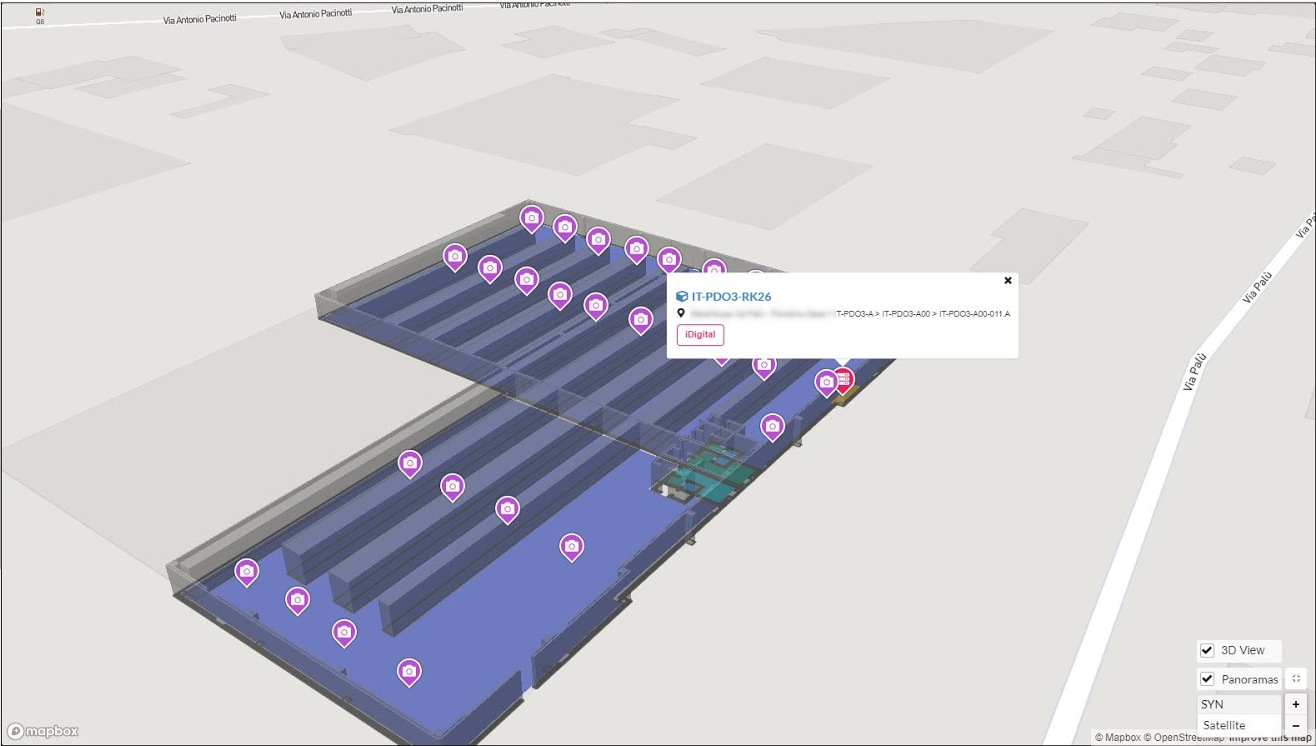
\includegraphics[height=5cm]{datasoil_assets_3dmap}
    \caption{Visualizzazione 3D di impianto produttivo con \textit{asset} mappati. Fonte: \href{https://datasoil.it/industry-40-smartcity-syn-asset-performance/auditing-inventory/}{Datasoil}}
\end{figure}
L'obiettivo è manipolare ed elaborare dati di natura inerentemente caotica, ordinarli e presentarli all'utente finale tramite interfacce grafiche intuitive (impiegando tecnologie all'avanguardia sia lato \textit{frontend} che lato \textit{backend}\footnote{\textit{Fronted} e \textit{backend} denotano, rispettivamente, la parte visibile all'utente di un programma e con cui egli può interagire (tipicamente un'interfaccia utente) e la parte che permette l'effettivo funzionamento di queste interazioni. {\tiny Fonte: \href{https://it.wikipedia.org/wiki/Front-end_e_back-end}{Wikipedia}}}).
\begin{figure}[H]
    \centering
    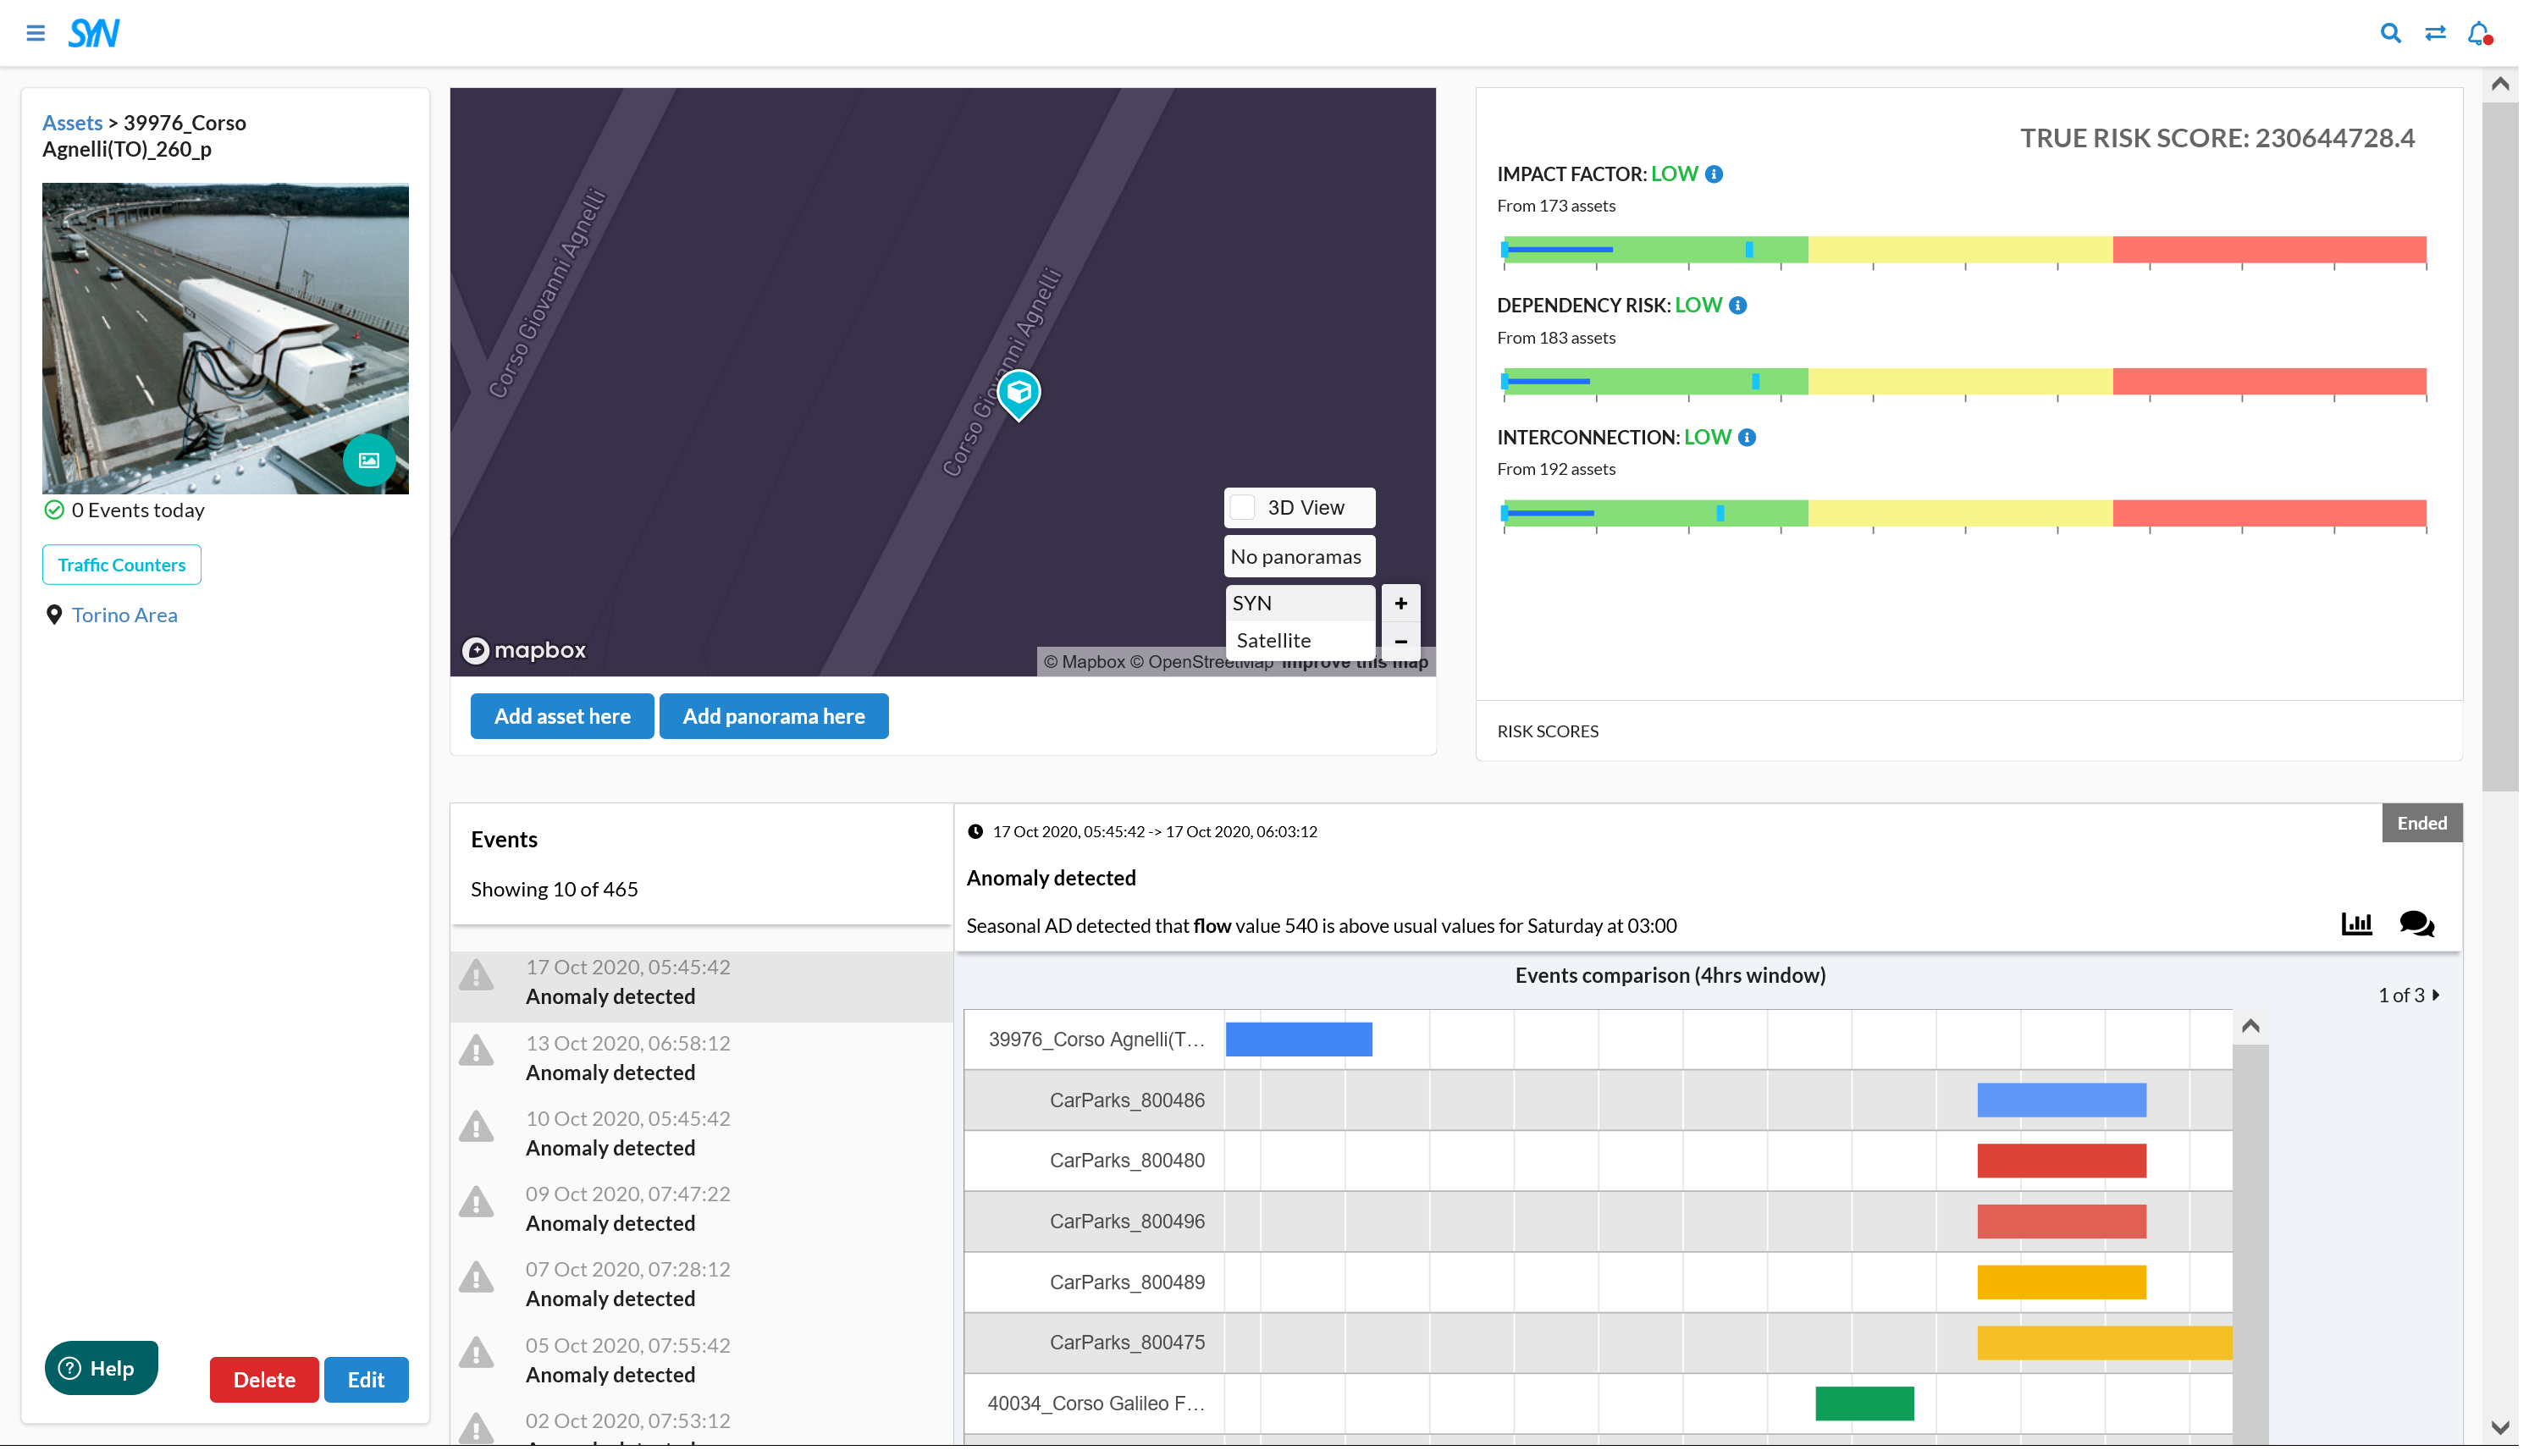
\includegraphics[width=\textwidth]{metriche_asset_datasoil}
    \caption{\textit{Screenshot} visualizzazione grafica di metriche di controllo per \textit{asset} aziendale.}
\end{figure}
Ho avuto modo di verificare molte di queste affermazioni direttamente tramite il progetto proposto, in quanto si tratta di un applicativo legato all'industria 4.0 che mappa \textit{asset} aziendali (come ad esempio macchinari) a un gemello digitale, permettendo sia di localizzarli su una mappa tridimensionale sia, obiettivo dello stage, di visualizzarli in realtà aumentata.

\subsection{Clientela}
\begin{figure}[H]
    \centering
    \includegraphics[height=5.5cm]{screenshot_home_datasoil}
    \caption{L'immagine scelta dall'azienda per il proprio sito mostra una chiara direzione aziendale. Fonte: \href{https://datasoil.it/industry-40-smartcity-syn-asset-performance/}{Datasoil}}
\end{figure}
Si evince da quanto discusso nella sezione precedente che l'offerta di Datasoil sia indirizzata a una clientela professionale, o meglio, aziendale, piuttosto che al mondo \textit{consumer}: 
l'applicazione sulla quale ho svolto lo Stage (MobileSYN) si occupa di gestione e controllo per \textit{asset} aziendali, e un altro prodotto da loro sviluppato, chiamato LifestyleSync, fornisce strumenti di monitoraggio della salute dei dipendenti, con \textit{app} di supporto "LSCoach" che permette a un allenatore di preparare allenamenti personalizzati e verificarne il progresso.\\
In sintesi Datasoil si focalizza su aziende industriali \textit{asset intensive} (ovvero con molti macchinari), manifatturiere e petrolifere, come ad esempio \href{https://www.stevanatogroup.com/it/}{Stevanato Group}.

\subsection{Processi interni}
L'azienda si serve di servizi noti e standardizzati per organizzare il lavoro e la comunicazione interna, ovvero Slack per la messaggistica, Meet per la comunicazione vocale a distanza, Jira per gestire il tracciamento delle \textit{issue} ("cose da fare" in ambito \textit{software}) e facilitare meccanismi agili di integrazione continua, e infine GitHub per quanto riguarda il controllo di versione.\\
Durante il progetto di stage che, per sua natura, è altamente sperimentale e ha quindi richiesto un approccio \textit{"trial and error"} ci si è limitati a usare una piccola Kanban Board di Jira per pianificare, per quanto possibile, il lavoro da svolgere.\\
L'azienda adotta un sistema di lavoro agile (come accennato sopra sfruttando Jira per applicare \textit{continuous delivery}) e fornisce anche ad associazioni esterne \textit{tutoring} riguardo a queste tematiche. 
\begin{figure}[H]
    \centering
    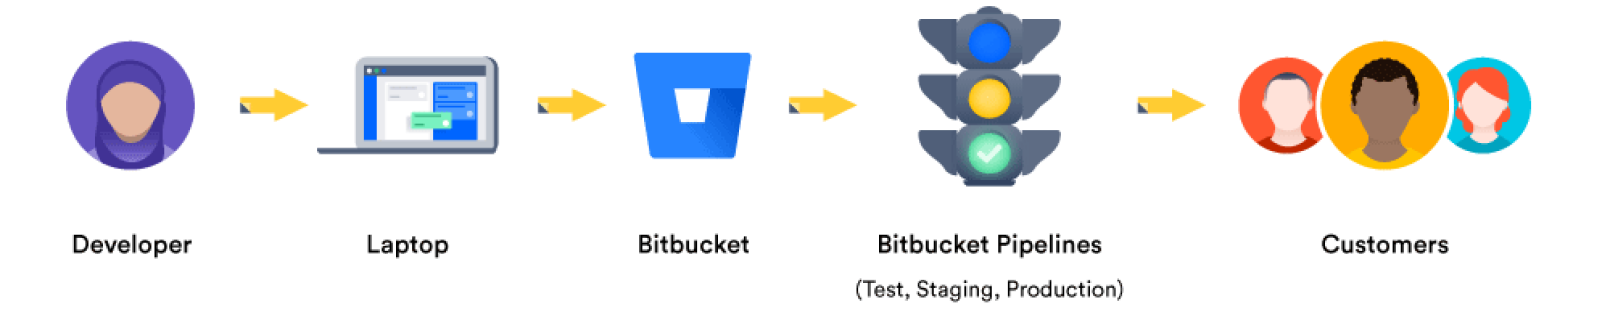
\includegraphics[width=\textwidth]{continuous-delivery-pipeline}
    \caption{\textit{Continuous delivery pipeline} tramite Jira. Fonte: \href{https://www.atlassian.com/continuous-delivery}{Atlassian}}
\end{figure}

%************************************************************************************************************
\section{Tecnologie e strumenti}
\label{sec:tecnologie-e-strumenti}
Di seguito vengono riportate le tecnologie e gli strumenti utilizzati durante il corso dello stage, divisi in due macrocategorie: di sviluppo (quindi legati strettamente alla produzione di \textit{software}) e organizzativi (più interessati alla gestione del codice prodotto e la comunicazione interna).\\
Verranno prima presentati singolarmente e in dettaglio, per poi mostrarne una visione d'insieme.

\subsection{Tecnologie e strumenti di sviluppo}
\subsubsection{Visual Studio Code}
\vsc{} è un \textit{editor} per codice sorgente, sviluppato da Microsoft servendosi del \textit{framework} Electron, disponibile per Windows, Linux e macOS. Le sue funzionalità comprendo supporto per \textit{debugging}, \textit{syntax highlighting}, \textit{intelligent code completion}, \textit{code refactoring}, e integrazione con Git. \\
Gli utenti possono configurare tema, \textit{macro}, preferenze e installare estensioni che ne aumentano le funzionalità aggiungendo ad esempio il supporto ai maggiori linguaggi di programmazione attualmente presenti.\\
Nella "Stack Overflow 2021 Developer Survey", \vsc{} è risultato essere l'IDE più popolare, adottato dal 70\% degli intervistati. {\tiny Fonte: \href{https://en.wikipedia.org/wiki/Visual_Studio_Code}{Wikipedia}}\\
E' inoltre presente e molto comoda l'estensione di Flutter che, tra le altre cose, permette di gestire direttamente nell'interfaccia i vari dispositivi (\textit{smartphone}, \textit{browser} o emulatore) sui quali installare e lanciare l'applicazione che si sta programmando.

\subsubsection{Android Studio}
\astudio{} è l'IDE (\textit{Integrated Development Environment}, ovvero un \textit{software} per facilitare la scrittura di codice) ufficiale del sistema operativo di Gooogle, sostituendo Eclipse dal 2015, costruito sul \textit{software} IntelliJ di JetBrains e progettato specificatamente per lo sviluppo Android. E' disponibile per Windows, Linux e macOS.\\
Il 7 maggio 2019 Kotlin rimpiazzò Java come linguaggio consigliato per Android, favorendo un'integrazione ancora maggiore con JetBrains che, appunto, ha sviluppato e prodotto Kotlin stesso.\\
Personalmente ho cercato nonostante tutto di programmare il più possibile su \vsc{} preferendolo quindi ad \astudio{} in virtù della sua maggiore leggerezza e delle sue più ampie possibilità di personalizzazione.

\subsubsection{Xcode}
Xcode è l'\ide{} per macOS, utilizzato obbligatoriamente per sviluppare \textit{software} per macOS, iOS, iPadOS, watchOS e tvOS.\\
Supporta codice sorgente i seguenti linguaggi: C, C++, Objective-C, Objective-C++, Java, AppleScript, Python, Ruby, ResEdit (Rez), e Swift (quest'ultimo è per noi di particolare interesse).\\
In generale è un \ide{} molto impopolare e viene percepita con grande frustrazione la sua obbligatorietà per lo sviluppo all'interno dell'ecosistema Apple. Personalmente mi sento allineato alla negativa opinione generale, complice soprattutto la scarsa responsività del programma.


\subsubsection{Dart}
Dart è un linguaggio di programmazione sviluppato da Google per il \textit{client development}, ovvero per applicazioni \textit{web} e \textit{mobile}, e può anche essere impiegato per la costruzione di applicazione \textit{desktop} e \textit{server}.\\
E' un linguaggio orientato agli oggetti, basato su classi, \textit{garbage-collected}, fortemente tipizzato e con una sintassi nello stile di C. Può compilare sia codice macchina che JavaScript e supporta interefacce, \textit{mixins}, classi astratte, \textit{refined generics} e inferenza di tipo.\\
Personalmente l'ho trovato elegante e conciso nella sua struttura, e presenta dei vantaggi consistenti come le espressioni ternarie e la \textit{null safety} (ovvero i valori di tipo \textit{null} devono essere esplicitati con sintassi specifiche che riducono enormemente la possibilità di incontrare errori a tempo di esecuzione).

\subsubsection{Flutter}
Flutter è un \textit{framework open-source} creato da Google per lo sviluppo dell'interfaccia utente di applicazioni multipiattaforma per Android, iOS, Linux, macOS, Windows, Google Fuchsia e il \textit{web} partendo da un singolo \textit{codebase} (collezione di \textit{file} sorgente necessari a ottenere un \textit{software} completo e funzionante).\\
Rilasciato a maggio 2017, le applicazioni in Flutter sono scritte in Dart e sfruttano molte delle funzionalità avanzate del linguaggio. Le componenti principali del \textit{framework} sono:
\begin{itemize}
    \item \textbf{Dart platform:} Flutter gira all'interno della Dart Virtual Machine, che si serve di un \textit{execution engine just-in-time};
    \item \textbf{Flutter engine:} scritto primariamente in C++, fornisce supporto a basso livello per il \textit{rendering} e implementa accessibilità, \textit{file} e \textit{network input/output}, supporto nativo per i \textit{plugin} e molto altro;
    \item \textbf{Foundation library:} scritta in Dart, fornisce classi e funzioni di base che vengono usate per costruire gli applcativi in Flutter, come ad esempio le \textit{Application Programming Interfaces} per la comunicazione con l'\textit{engine};
    \item \textbf{Design-specific widgets:} Flutter contiene due famiglie di \textit{widget} che si conformano a delle specifiche scuole di \textit{design}: "Material" per Google e "Cupertino" per Apple;
    \item \textbf{Flutter DevTools:} famiglia di strumenti generici che vengono sfruttati per lo sviluppo di \textit{software} in Flutter.
\end{itemize}
~\\
Inoltre, una libreria fondamentale per semplificare l'utilizzo di Flutter è "Flutter Hooks": lo scopo è implementare delle strutture simili agli Hooks di React, che consentono di sostituire gli "Stateful Widget" riducendo la quantità di codice ripetuto e semplificando la gestione del ciclo di vita dei \textit{widget} grazie alla funzione "useEffect".

\subsubsection{Java}
Java è un linguaggio di programmazione ad alto livello orientato agli oggetti progettato per avere il minor numero possibile di dipendenze implementative (favorendo quindi l'uso di interfacce e classi astratte) e, soprattutto, per aderire al motto \textit{"write once, run anywhere"}: il \textit{bytecode} di Java può infatti girare senza necessità di ricompilazione su qualsiasi piattaforma che supporti la Java Virtual Machine (comunemente abbreviata in JVM).\\  
La sintassi è simile a quelle di C o C++, ma fornisce funzionalità dinamiche generalmente inedite per i linguaggi compilati, come \textit{reflection} (un programma in esecuzione può modificare se stesso) e modifica del codice a \textit{runtime}.\\
Originalmente rilasciato nel 1995 come componente centrale della piattaforma Java per Sun Microsystems e sotto licenza proprietaria, dal 2007 la maggior parte dei suoi componenti sono diventati \textit{open-source} sotto l'ombrello della "GPL-2.0-only" (licenza specifica per \textit{software} libero pubblicata dalla Free Software Foundation).\\
Sebbene Oracle (attuale proprietario di Sun Microsystems) offra un'implementazione proprietaria chiamata "HotSpot JVM", la specifica ufficiale è la "OpenJDK JVM" che è gratuita, \textit{open-source} e predefinita nella maggior parte delle distribuzioni Linux.

\subsubsection{Kotlin}
Kotlin è un linguaggio di programmazione multipiattaforma staticamente tipizzato. Progettato per avere completa interoperabilità con Java, gode di una sintassi più concisa di quest'ultimo grazie all'inferenza di tipo di cui è dotato. Dipende dalla Java Class Library per la versione della Java Virtual Machine da usare.\\
E' inoltre in grado di compilare codice in JavaScript (sfruttato poi da applicazioni \textit{frontend}) o codice nativo tramite "LLVM" (per app iOS che condividono le logiche operative con applicazioni Android).\\
Incluso in Android Studio come alternativa al compilatore standard Java dal 2017, produce \textit{bytecode} Java 8 di default ma permette al programmatore di scegliere delle versioni successive (fino a Java 18).

\subsubsection{Swift}
Swift è un linguaggio di programmazione ad alto livello, compilato, sviluppato da Apple e dalla comunità \textit{open-source}.\\
Inizialmente rilasciato nel 2014, il suo scopo è rimpiazzare il precedente linguaggio di Apple Objective-C, ormai obsoleto visto che è rimasto largamente invariato dagli anni '80 ed è quindi manchevole di funzionalità moderne.\\
Swift lavora con i \textit{framework} Cocoa e Cocoa Touch, e un aspetto chiave del suo \textit{design} è l'interoperabilità con una grossa parte del codice esistente in Objective-C (che, naturalmente, permea l'ecosistema Apple) sfruttando la \textit{runtime library} di Objective-C (che permette anche di far girare C e C++).\\
E' stato costruito con il \textit{framework} di compilazione LLVM ed è stato incluso in Xcode dalla sesta versione, rilasciata nel 2014.

\subsubsection{Azure Spatial Anchors}
Azure Spatial Anchors è un servizio di Microsoft mirato a fornire strumenti per sviluppare applicazioni in realtà aumentata su dispositivi iOS o Android predisposti per, rispettivamente, ARKit e ARCore, oppure su Microsoft HoloLens.\\
Permette di riconoscere spazi tridimensionali all'interno dei quali posizionare punti di interesse, chiamati Spatial Anchors, che possono essere salvati in \textit{cloud} e poi recuperati, e possono essere messi in relazione a oggetti reali (come macchinari in un contesto industriale) o virtuali.

\subsubsection{ARCore}
ARCore, conosciuto anche come Google Play Services per AR, è un \sdk{} (generalmente abbreviato in SDK) prodotto da Google per permettere lo sviluppo di applicazioni in realtà aumentata.\\
Si serve di tre componenti principali:
\begin{itemize}
    \item \textbf{6DOF:} il dispositivo sfrutta una piattaforma inerziale a sei assi per comprendere e tracciare la propria posizione relativa allo spazio;
    \item \textbf{Environmental understanding:} permette riconoscere dimensioni e locazione delle superfici lisce;
    \item \textbf{Light estimation:} permette al telefono di stimare le condizioni di luce dell'ambiente.
\end{itemize}
\asa{} si appoggia proprio ad ARCore per implementare le proprie funzionalità di realtà aumentata su Android.

\subsubsection{ARKit}
ARKit è la controparte Apple di ARCore, ovvero è un \sdk{} che permette lo sviluppo di applicazioni in realtà aumentata su dispositivi Apple.\\
Combina i dati del dispositivo di tracciamento spaziale (come la piattaforma inerziale a sei assi) con un \textit{processing} avanzato della scena ripresa per fornire un'esperienza in realtà aumentata convincente.\\
Indubbiamente migliore di ARCore, produce risultati più fluidi (inteso come effettiva fluidità percepita guardando la scena attraverso il dispositivo), meglio implementati con le tecnologie esistenti e risparmia al programmatore molti oneri (come la gestione delle sessioni) occupandosene direttamente in modo autonomo.

\subsubsection{Visione d'insieme}
\vsc{} è un \textit{editor} per codice sorgente che permette grande estensibilità tramite \textit{plugin} appositi che, per il progetto, ho configurato in modo tale da aggiungerci la compatibilità con il \textit{framework} utilizzato per lo sviluppo \textit{mobile}, ovvero Flutter, che si appoggia sul linguaggio Dart. Quest'ultimo è un linguaggio orientato agli oggetti e fortemente tipizzato che nasce per la creazione di interfacce grafiche \textit{frontend mobile}. Integrando Flutter in \vsc{} si ottengono vari vantaggi, come ad esempio la possibilità di gestire eventuali emulatori o dispositivi Android con facilità.\\
Essendo lo scopo del progetto l'integrazione di \asa{} (tecnologia per gestire ancoraggi in realtà aumentata) in un'applicazione Flutter, è stato necessario studiare anche gli \sdk{} sui quali si appoggia il servizio di Microsoft, ovvero ARCore (lato Android) e ARKit (lato iOS). \asa{} implementa tali funzionalità in linguaggi nativi, ovvero Java per Android e Swift per iOS, il che ha portato la necessità a utilizzare due \ide{}(abbreviato in IDE) ulteriori a \vsc{}: Xcode e Android Studio.\\
Xcode è obbligatorio per programmare in Swift, mentre Android Studio da un grosso aiuto al programmatore quando lo usa per sviluppare applicazioni Android in Java o Kotlin (linguaggio che si è dovuto utilizzare per \aplug{}, ovvero il \textit{framework} ultimamente selezionato che tratteremo nel terzo capitolo di questo documento).
\begin{figure}[H]
    \textbf{Strumenti di sviluppo e rispettivi linguaggi:}
    \begin{center}
    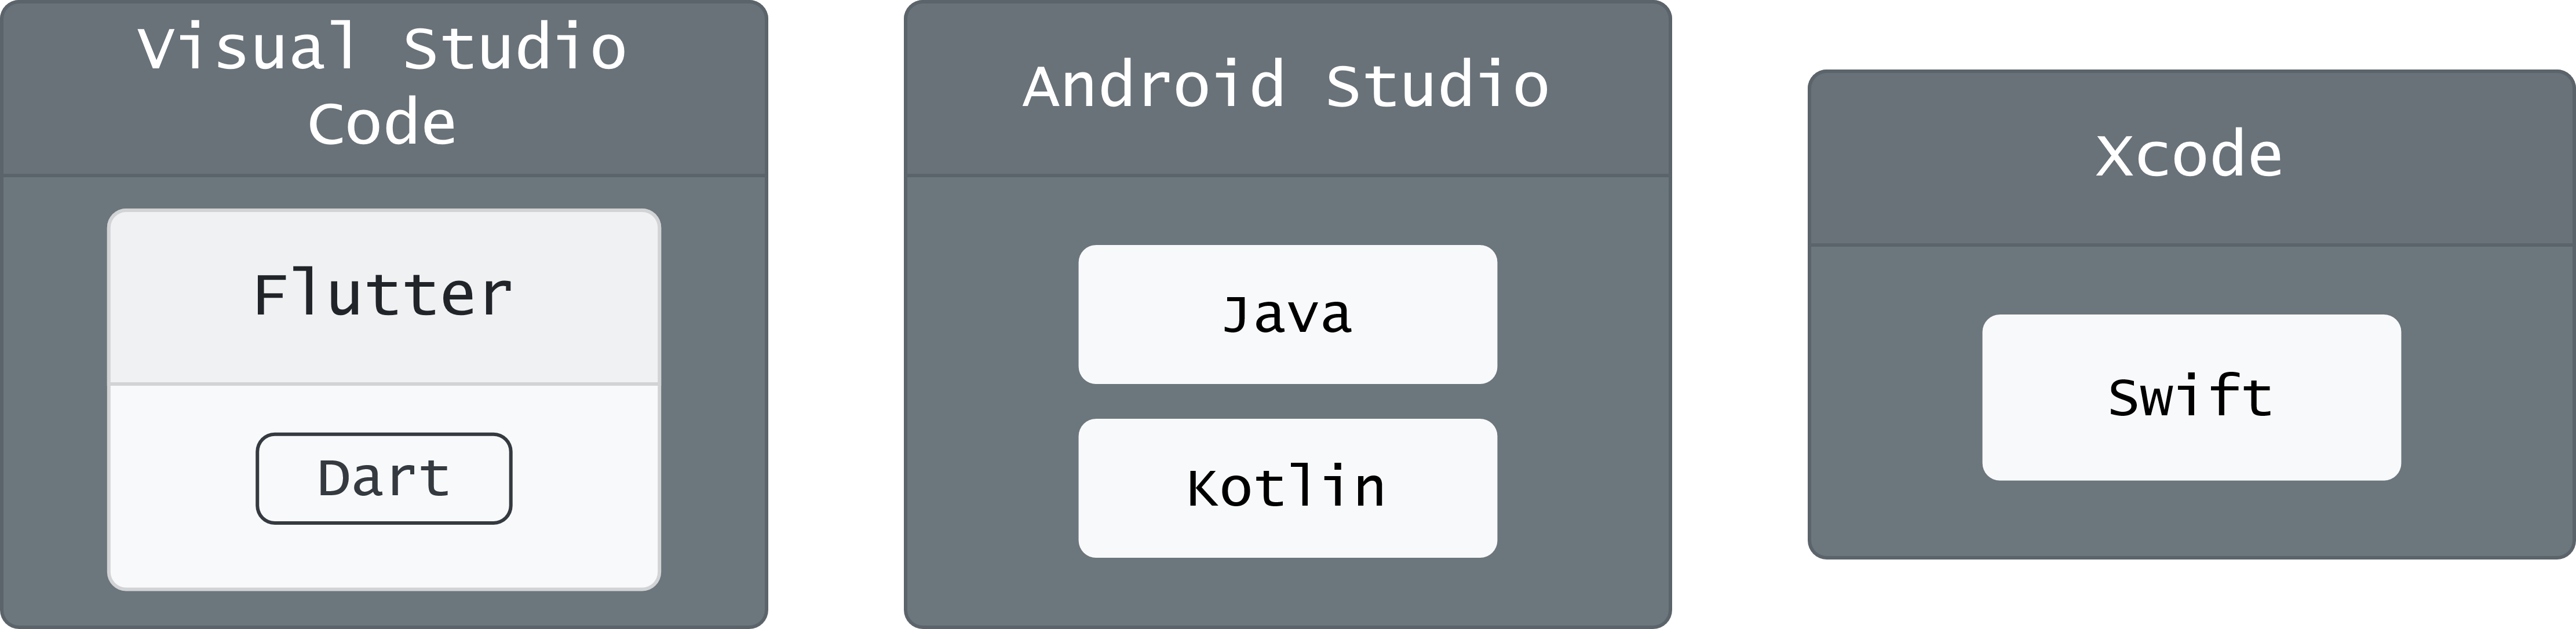
\includegraphics[height=3cm]{ides}
    \caption{\textit{Integrated development environments} e linguaggi per i quali sono stati usati}
    \end{center}
\end{figure}

\begin{figure}[H]
    \textbf{Tecnologie realtà aumentata, linguaggi e sistemi operativi:}
    \begin{center}
    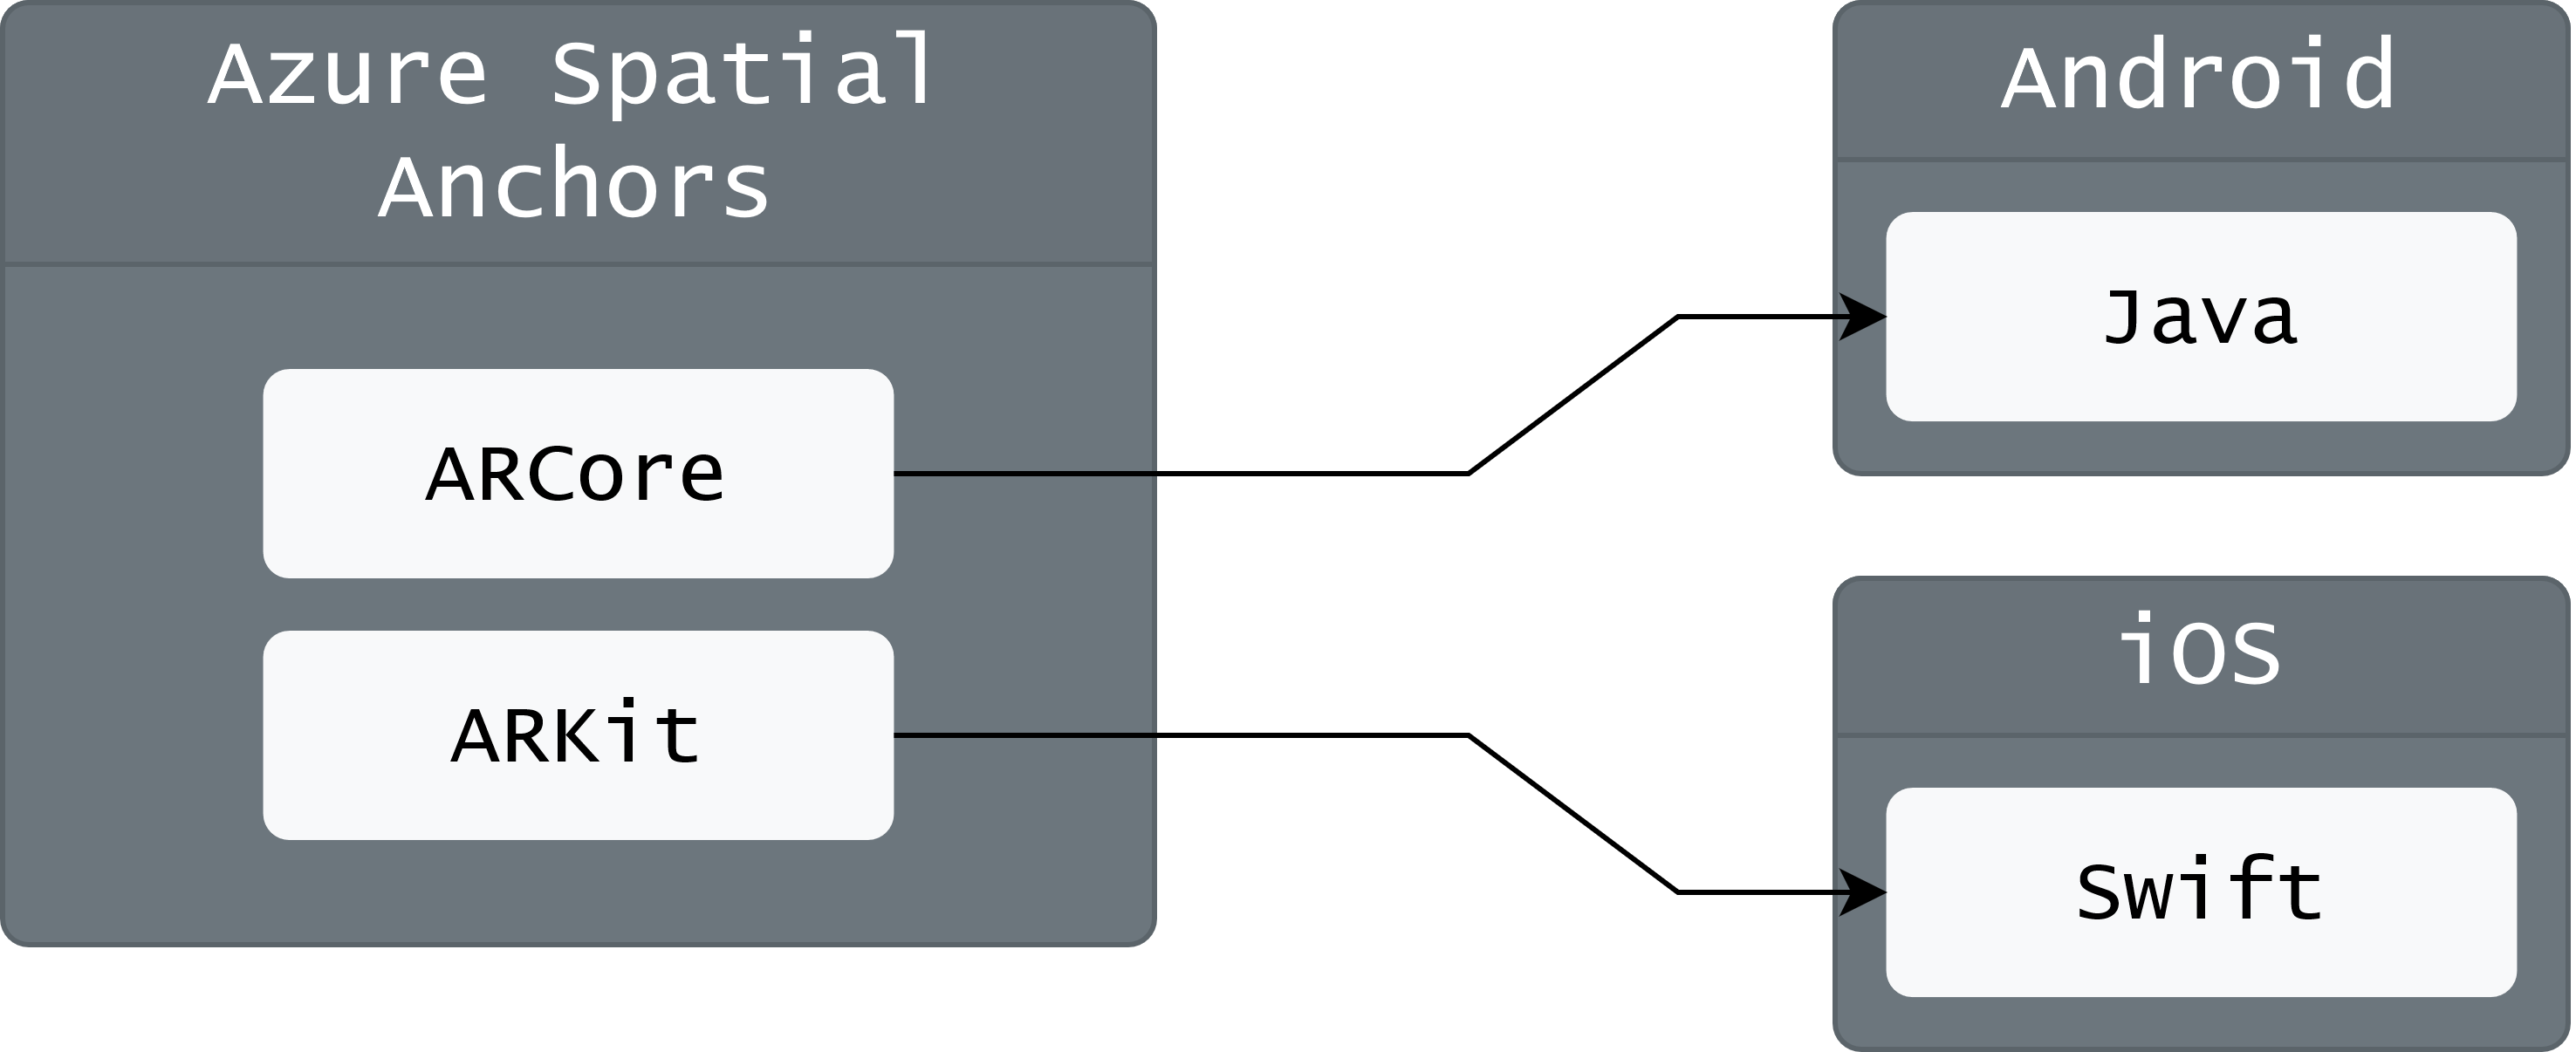
\includegraphics[height=3.5cm]{tecASA}
    \caption{\asa{} e linguaggi nativi utilizzati per implementare le sue componenti in Android e iOS}
    \end{center}
\end{figure}

\begin{figure}[H]
    \textbf{\textit{Framework} scelto e sua relazione con tecnologie e linguaggi:}\\
    In questo caso il \textit{framework} ha le componenti native scritte in Kotlin che è compatibile nativamente con Java e funge quindi da contenitore (\textit{"wrapper"}) per quest'ultimo.\\
    \begin{center}
    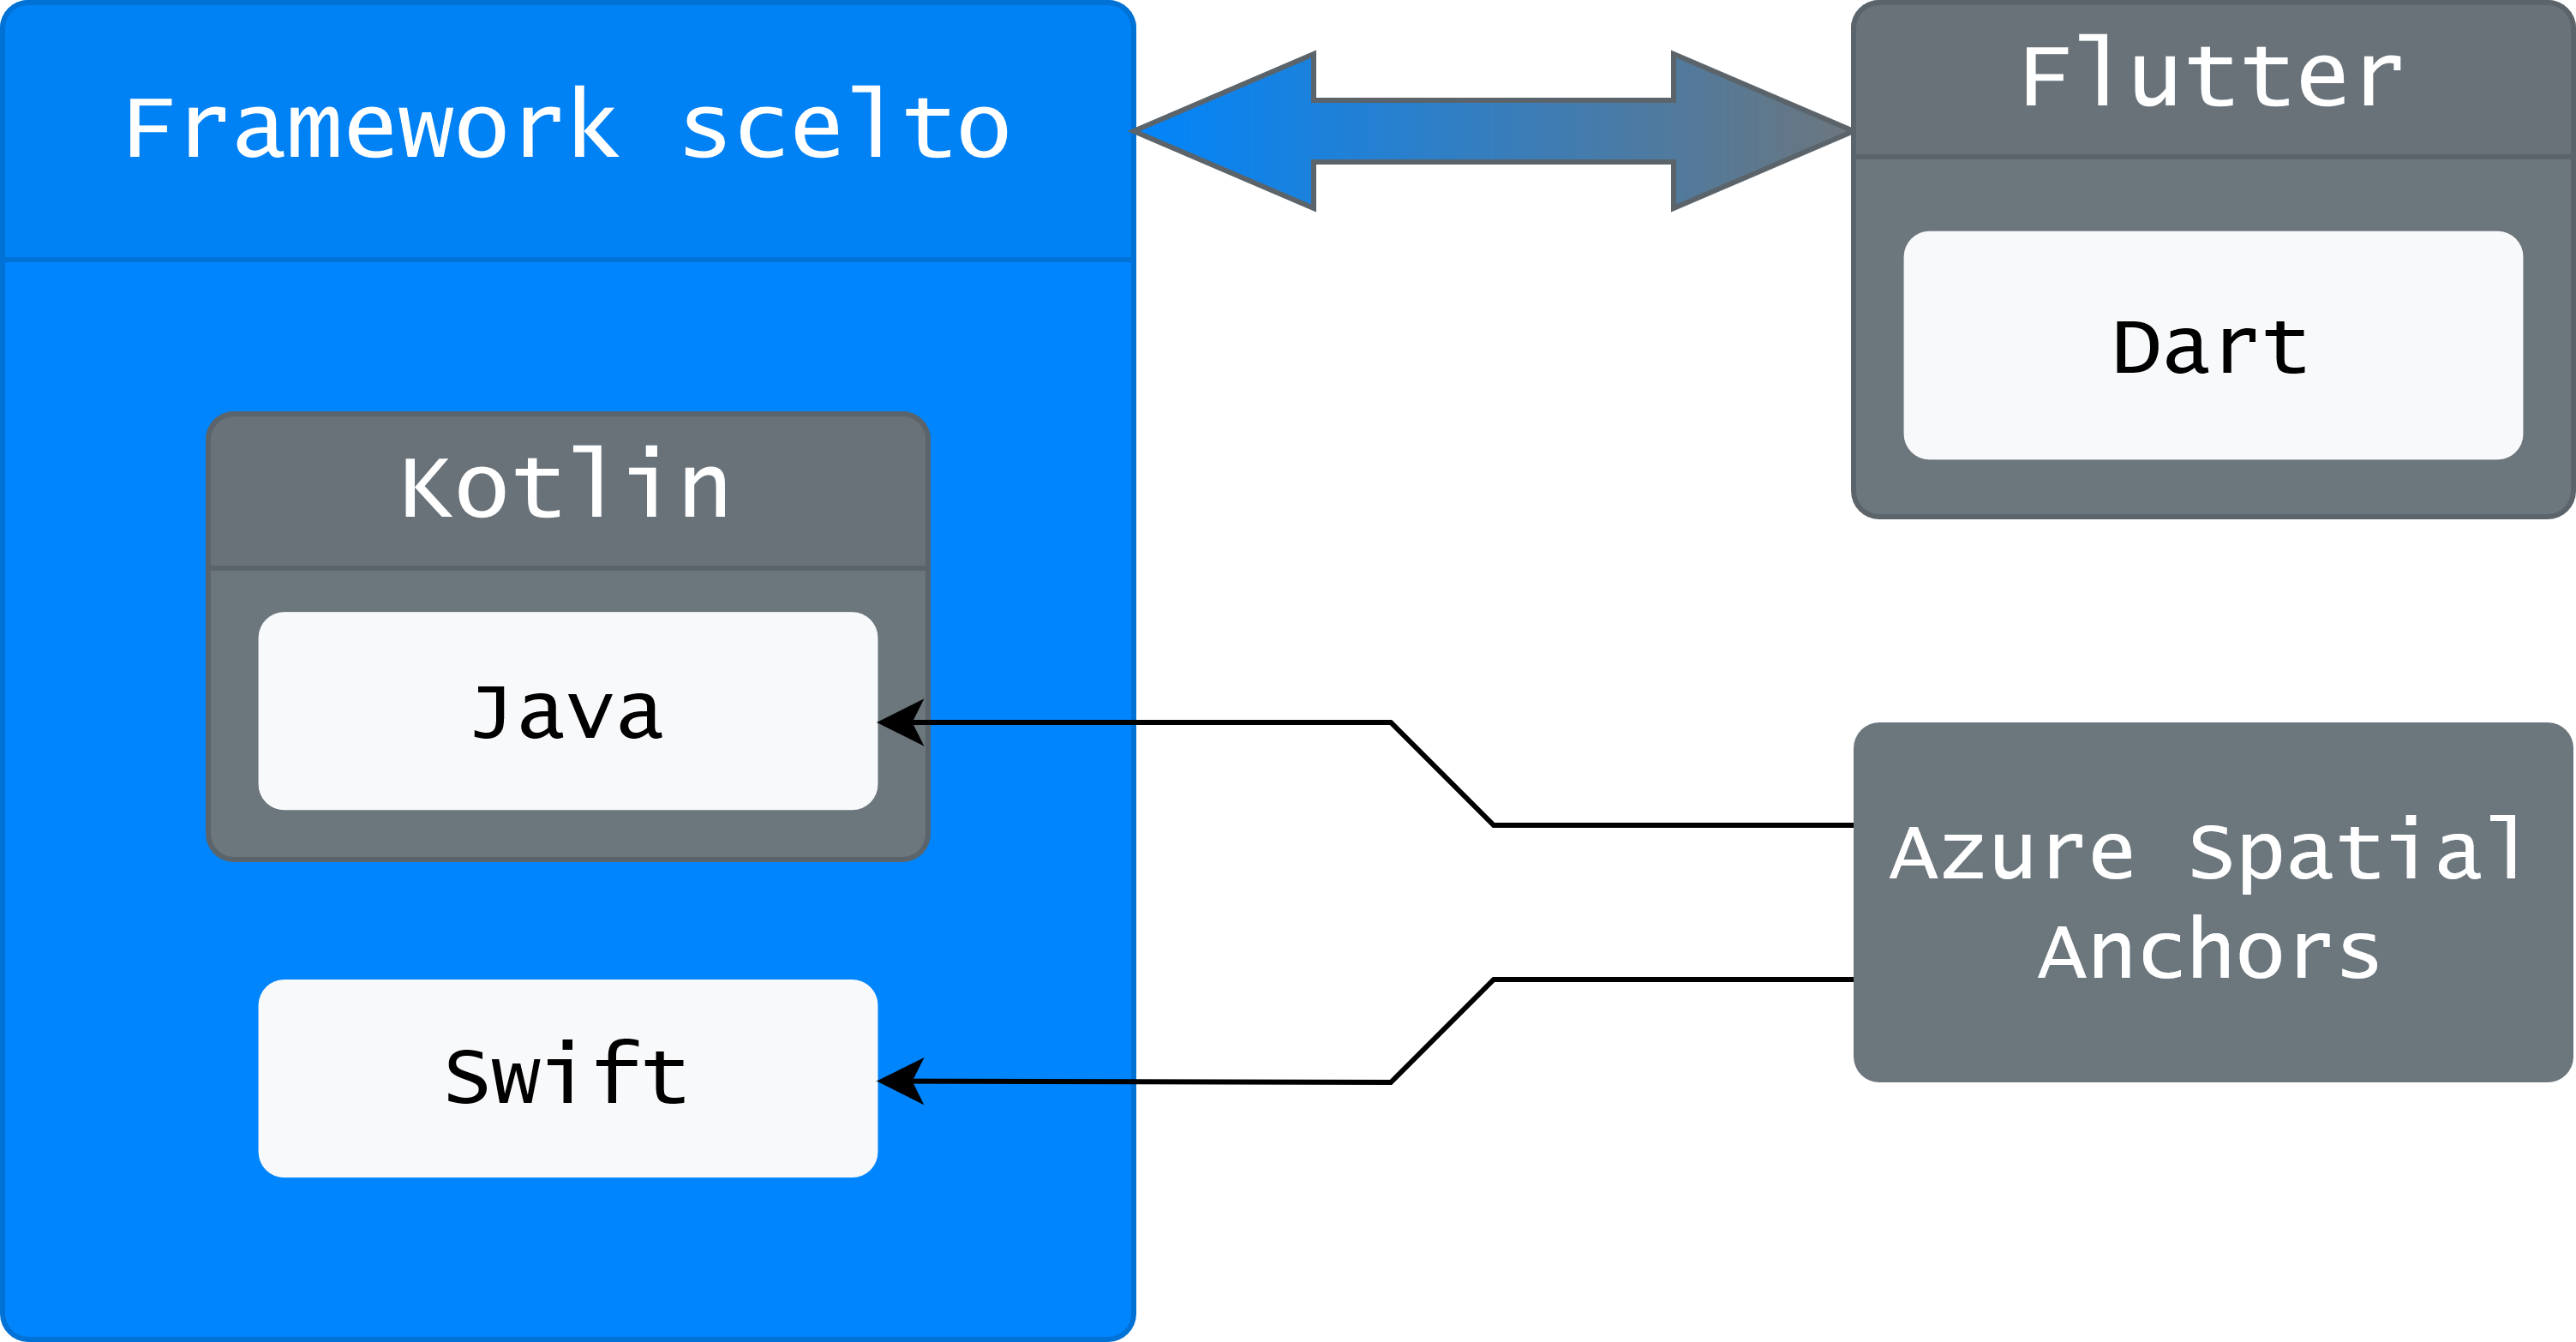
\includegraphics[height=4.5cm]{aplug_linguaggi}
    \caption{Il \textit{framework} selezionato comunica con Flutter e implementa delle componenti native alle quali si interfacciano le \asa{}}
    \end{center}
\end{figure}
%**************************************************************
\subsection{Strumenti organizzativi}
\subsubsection{Slack}
Slack è una piattaforma di comunicazione istantanea di proprietà di Salesforce e sviluppata da Slack Technologies per Windows, Linux, macOS, Android e iOS.\\
Permette di comunicare tramite messaggi, chiamate vocali e video, e di inviare \textit{media} e \textit{files} nelle \textit{chat} private o nei canali. Quest'ultimi fungono da aggregatori e permettono di suddividere tematicamente la comunicazione.\\
E' inoltre possibile suddividere a un livello ancora più alto tramite i \textit{workspaces}, che aggregano al proprio interno utenti, canali e applicazioni: sono proprio quest'ultime che mostrano con maggiore chiarezza l'orientamento aziendale di Slack, che infatti fornisce integrazione nativa con i maggiori software gestionali e organizzativi (come ad esempio Jira, Zoom, Drive, Outlook, etc).

\subsubsection{Github}
GitHub è il più grande servizio di \textit{hosting} di codice sorgente al mondo, abitualmente usato per sviluppare progetti \textit{open-source}, e fornisce vari servizi: controllo di versione tramite Git distribuito e \textit{access control}, \textit{bug tracking}, \textit{issue tracking}, richieste di modifiche \textit{software}, \textit{task management}, integrazione continua e \textit{wiki} per ogni progetto.\\ 
Permette inoltre, tramite \textit{forking}, \textit{pull request} e commenti, il miglioramento collaborativo del \textit{software}, ad esempio risolvendo errori, aggiungendo funzionalità o migliorando quelle presenti.

\subsubsection{Jira}
Jira è un \textit{software} proprietario sviluppato da Atlassian che si occupa di fornire una piattaforma potente e funzionale di \textit{bug} e \textit{issue tracking}, presentando il tutto tramite interfacce grafiche chiare e complete. Favorisce inoltre la pianificazione e la collaborazione all'interno dei \textit{team} utilizzando, oltre alle \textit{issues}, anche \textit{tasks} e \textit{user stories}.\\
Fornisce inoltre \textit{template} già pronti per implementare i più noti \textit{framework} di lavoro come Scrum e Kanban.\\
Jira mira inoltre a ottimizzare il flusso di lavoro e favorire un miglioramento continuo fornendo visualizzazioni espressive di metriche per tenere traccia dei tempi di sviluppo e scoprire colli di bottiglia.

\subsubsection{Visione d'insieme}
Presentiamo ora gli strumenti organizzativi in relazione tra loro e con quelli di sviluppo, assieme a descrizione minimale. Per approfondire i singoli elementi si rimanda alle sezioni immediatamente successive.\\
Per quanto riguarda la comunicazione diretta interna all'azienda, che sia condividere documenti, frammenti di codice o domande di vario tipo, lo strumento scelto è Slack (piattaforma di messaggistica orientata alle aziende).\\
Tutto il codice per tutte le tecnologie affrontate (applicazione MobileSYN, esempi ufficiali \asa{}, \textit{framework} selezionato) è contenuto in GitHub, che fornisce sia \textit{hosting} che controllo di versione. Infine per organizzare quanto possibile i lavori si è scelto di utilizzare Jira (\textit{software} proprietario di \textit{issue tracking}), che è anche integrato in Slack.\\
\begin{figure}[H]
    \centering
    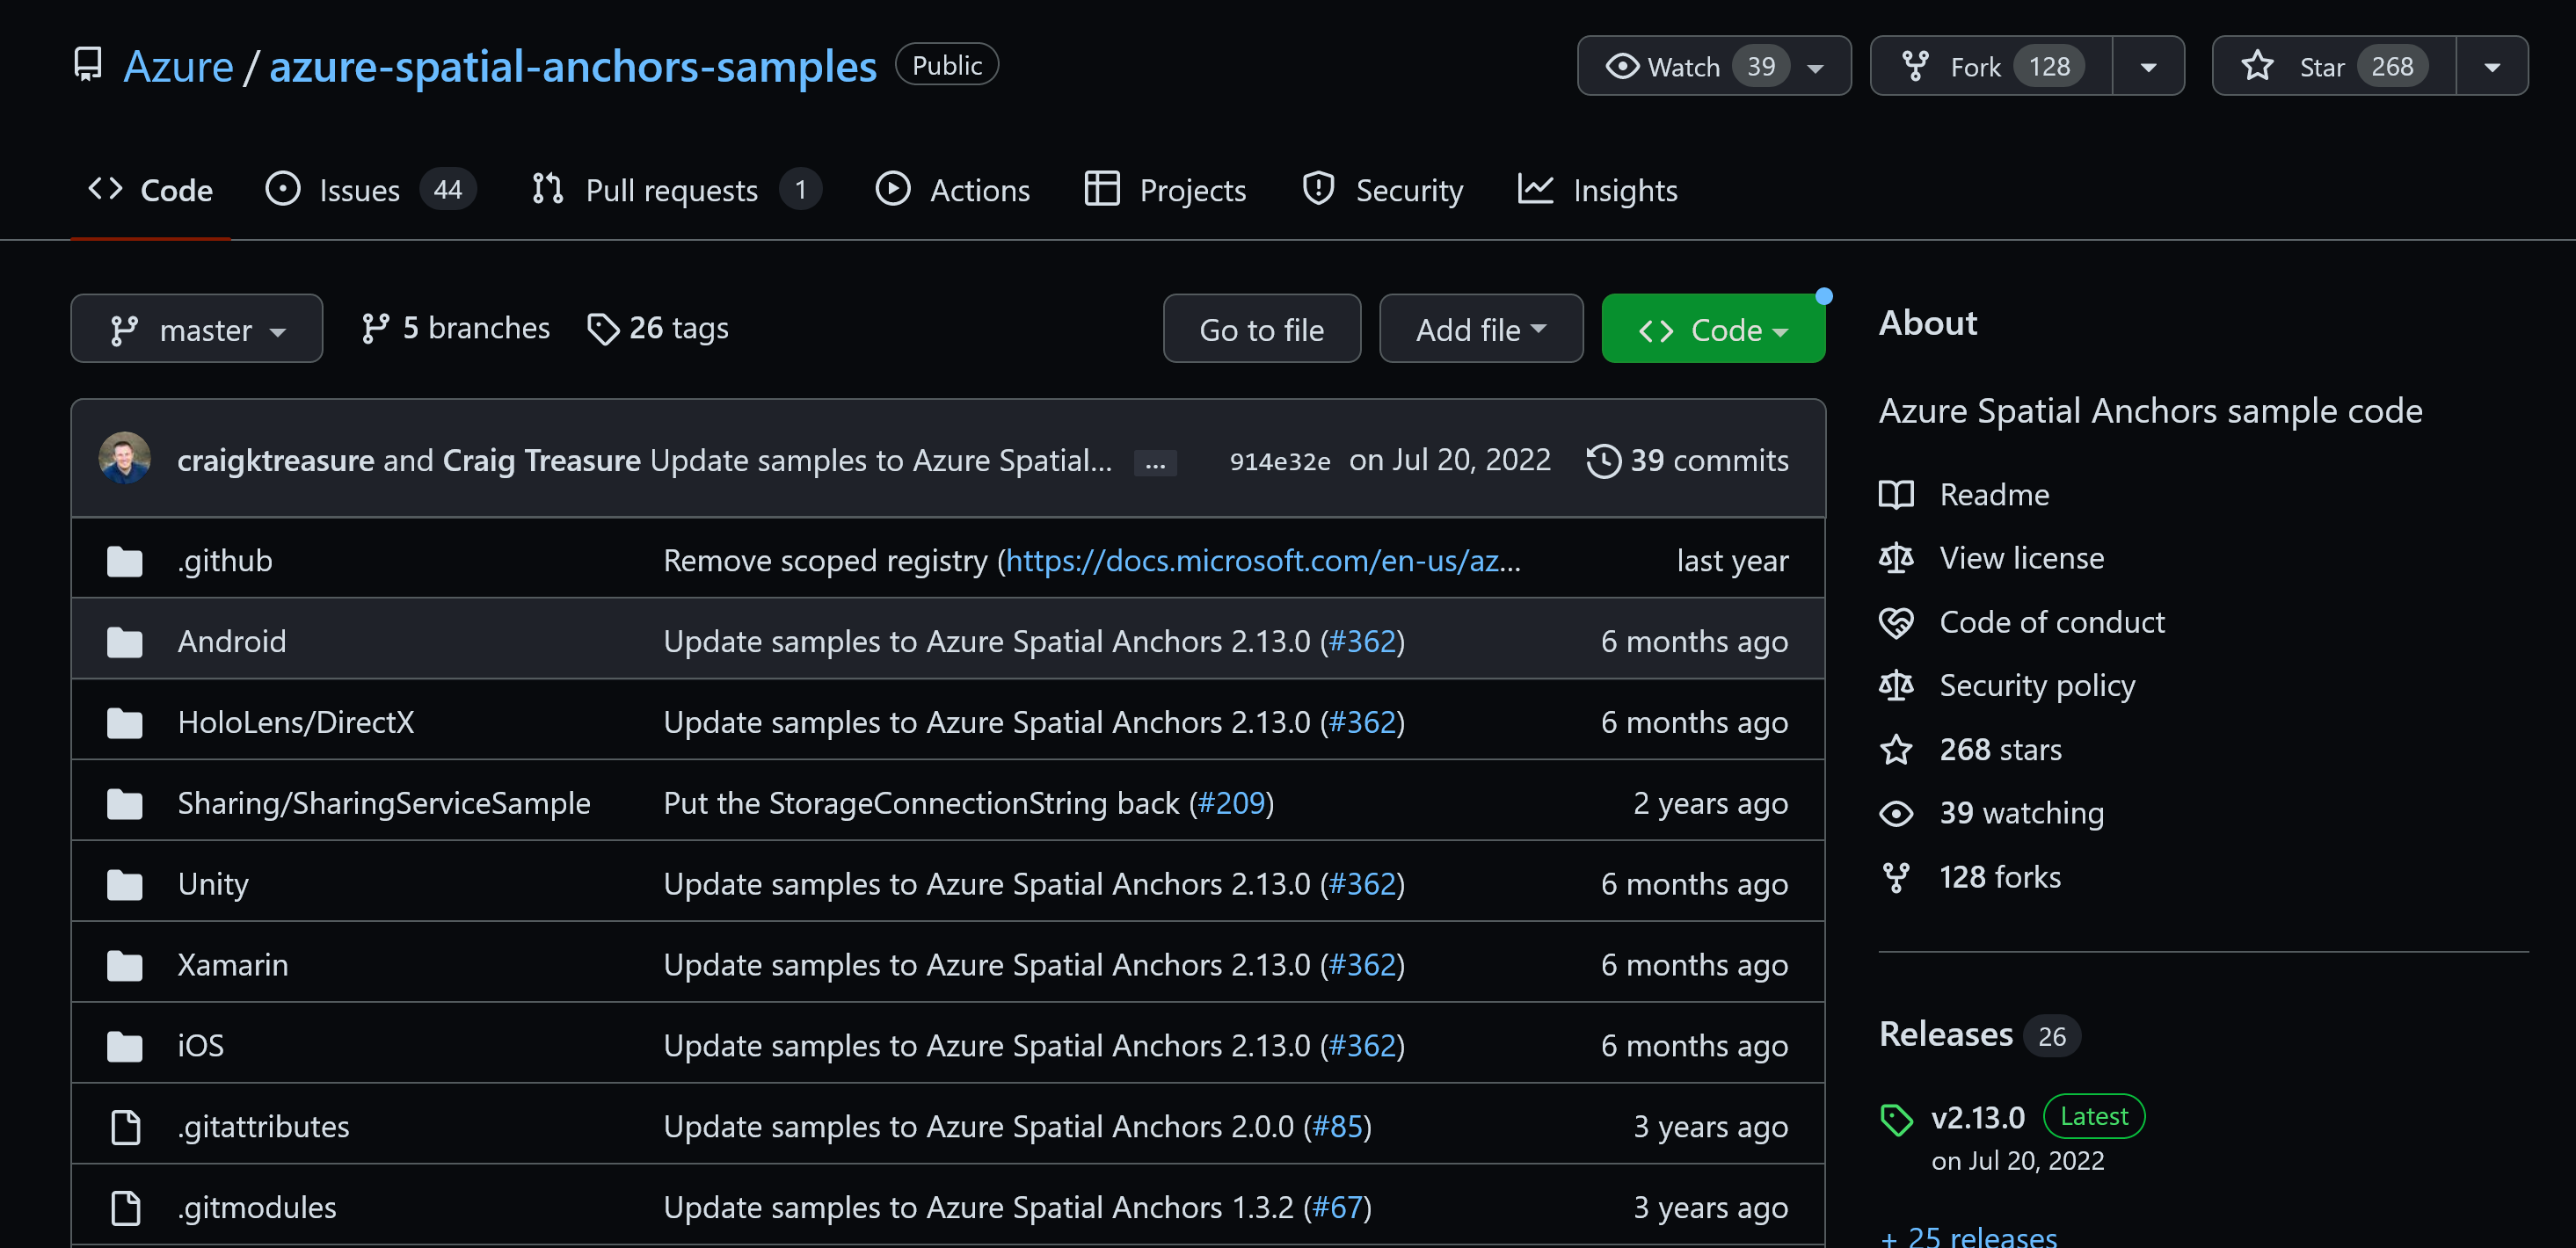
\includegraphics[width=\textwidth]{asa_github_screen}
    \caption{Il codice per l'applicazione di esempio ufficiale di \asa{} è interamente contenuta in \href{https://github.com/Azure/azure-spatial-anchors-samples}{questa} \textit{repository} di GitHub}
\end{figure}

\section{Innovazione, stage e prodotti}
E' immediatamente evidente guardando le tecnologie impiegate che Datasoil pone particolare attenzione sul tema dell'innovazione: lato \textit{backend} troviamo servizi \aws{} impiegati per decentralizzare la gestione del \textit{server} (ad esempio S3), e ovviamente il già citato \asa{}, mentre lato \textit{frontend}\footnote{Collezione di codice che fornisce funzionalità generiche che possono essere sovrascritte, specializzandole, per adattarle agli scopi voluti. Sono simili alle librerie se visti come astrazioni riutilizzabili di codice incluso in APIs (\textit{Application Programming Interfaces}, permettono a due o più componenti \textit{software} di comunicare) ben definite, tuttavia ciò che le differenzia è che il controllo di esecuzione non è dettato dal chiamante, ma dal \textit{framework} stesso. E' proprio questa inversione di controllo la caratteristica principale dei \textit{framework}.} vediamo l'impiego di linguaggi di programmazione e \textit{framework} recenti come Dart e Flutter (usati per sviluppare tutt i prodotti in campo \textit{mobile}).\\
E' bene sottolineare, però, che gli strumenti scelti non sono stati selezionati solo per rincorrere un ideale di avanguardia: hanno infatti tutti alle spalle delle grosse corporazioni (Amazon nel caso di \aws{}, Microsoft nel caso di \asa{} e Google nel caso di Dart e Flutter) che garantiscono loro un certo grado di stabilità e sicurezza.\\
L'attenzione all'innovazione mostrata da Datasoil si riflette sia negli \textit{stage} proposti che nei prodotti e servizi direttamente offerti dall'azienda: ad esempio nell'uso di HoloLens per implementare funzioni di realtà aumentata oppure nelle sessioni di \textit{tutoring} per terzi (riguardo appunto queste tecnologie o pratiche di sviluppo agile) che i \textit{senior} svolgono a cadenza regolare.
\begin{figure}[H]
    \centering
    \begin{minipage}{.5\textwidth}
      \centering
      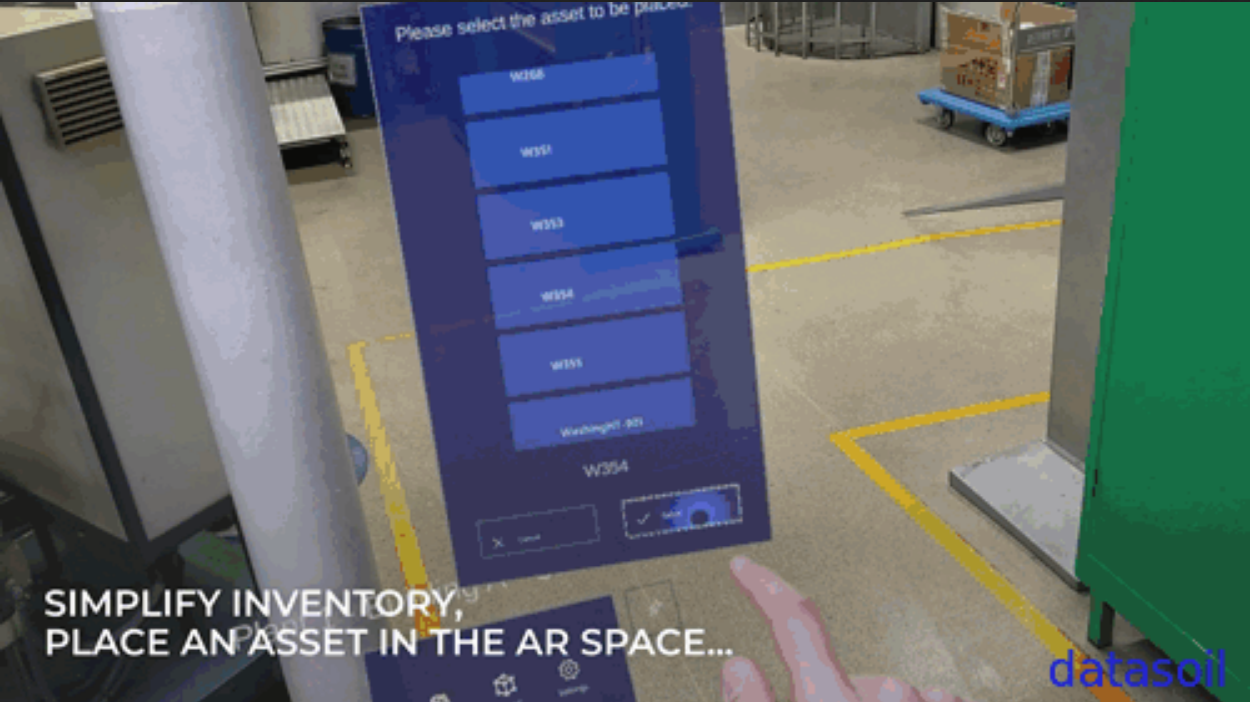
\includegraphics[width=1\linewidth]{hololens1_datasoil}
      \captionof{figure}{Menù HoloLens}
      \label{fig:test1}
    \end{minipage}%
    \begin{minipage}{.5\textwidth}
      \centering
      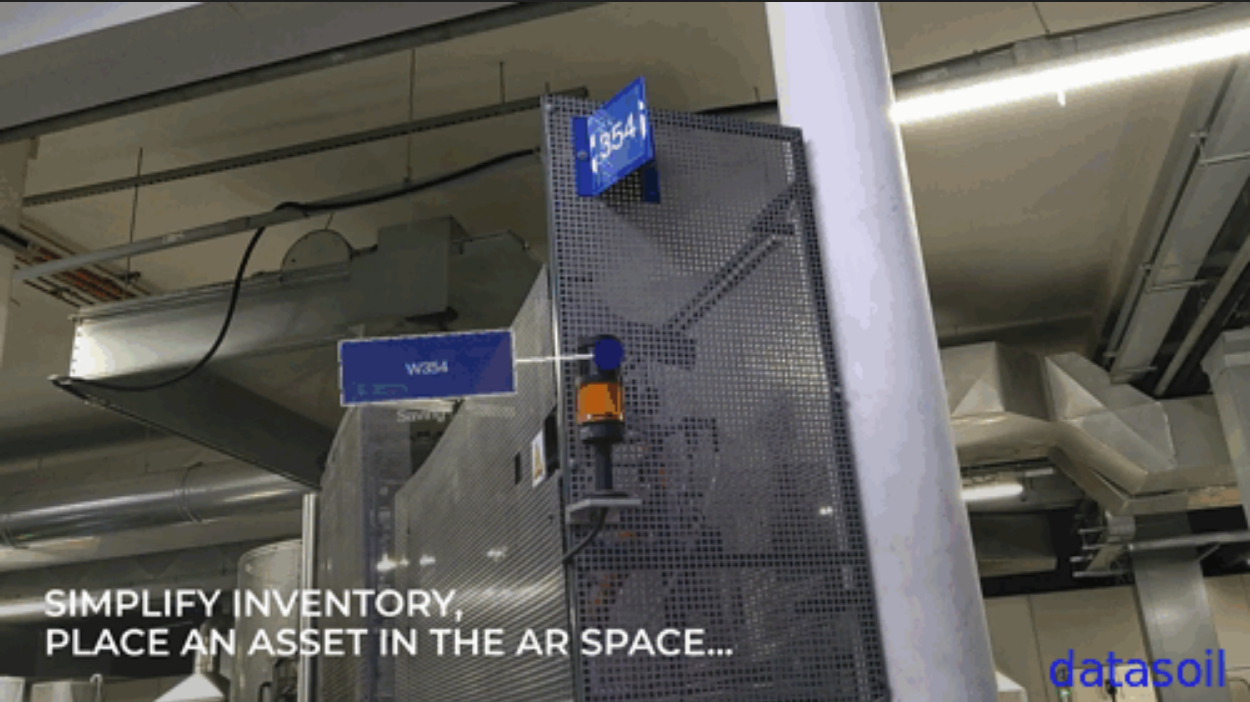
\includegraphics[width=1\linewidth]{hololens2_datasoil}
      \captionof{figure}{Posizionamento \textit{asset}}
    \end{minipage}
    \caption{HoloLens usato in azienda per gestire \textit{asset} in realtà aumentata. Fonte: \href{https://datasoil.it/industry-40-smartcity-syn-asset-performance/auditing-inventory/}{Datasoil}}
\end{figure}
Gli \textit{stage} riescono a essere innovativi sia direttamente che indirettamente: se si tratta di un progetto sperimentale vero e proprio lo è per sua stessa natura, tuttavia anche nel caso in cui l'obiettivo sia limitato a sviluppare funzioni in maniera più "meccanica", porta comunque lo studente ad avere a che fare con gli strumenti moderni che vengono impiegati giornalmente in azienda.\\
Vengono quindi integrati nel contesto aziendale in modalità duplice: a volte sono funzionali alla sperimentazione di nuove soluzioni, altre volte sono già inquadrati in una \textit{pipeline} produttiva (ad esempio potrebbero trattare lo sviluppo di alcune pagine di un'applicazione \textit{mobile}). Anche nel primo caso però se ciò che è stato prodotto risulta interessante per dei possibili clienti viene portato avanti e integrato anche quando lo \textit{stage} si è ormai concluso.
